%! TEX program = pdflatex

\documentclass[oneside,solution]{karazin-complan-assign}

\usepackage[utf8]{inputenc}
\usepackage[english,ukrainian]{babel}

\usepackage{mathtools}

\let\Im\relax
\DeclareMathOperator{\Im}{Im}
\let\Re\relax
\DeclareMathOperator{\Re}{Re}

\usetikzlibrary{decorations.markings,positioning}

\providecommand{\poles}{
  \node (poles) at (2.5,1.5) {poles of $h(p_0)$};
  \draw[fill]
  (1.5,3) coordinate [circle,fill,inner sep=1pt,label=right:$p_1$] (p1)
  (2,-2) coordinate [circle,fill,inner sep=1pt,label=below:$p_2$] (p2)
  (-3,1) coordinate [circle,fill,inner sep=1pt,label=above:$p_3$] (p3)
  (-2,-1.5) coordinate [circle,fill,inner sep=1pt,label=above:$p_4$] (p4);
  \draw[ultra thin,gray] (poles) -- (p1) (poles) -- (p2) (poles.west) -- (p3) (poles) -- (p4);
}

\def\xr{3.5}
\def\yr{3}


\title{Домашня робота}
\author{Захаров Дмитро}
\studentID{МП-31}
\instructor{Гиря Н.П.}
\date{\today}
\duedate{23:59 14 квітня, 2024}
\assignno{4}
\semester{Весняний семестр 2024}
\mainproblem{Відображення \#1. Варіант 5}

\begin{document}

\maketitle

% \startsolution[print]

\problem{Лінійно-дробове відображення}

\hspace{20px}\textbf{Умова.} Знайти образ області $\mathcal{D}$ при відображенні $\omega$, знайти нерухомі точки кожного відображення, вказати хоча б одну пару симетричних точок в кожному завданні.

\textbf{Пункт 1.}
\begin{equation*}
    \mathcal{D} = \{z \in \mathbb{C}: \text{Re}(z) > 3\}, \; \omega(z) = 5z-3i, \; \omega(z) = \frac{2}{z-1}
\end{equation*}

\textbf{Пункт 2.}
\begin{equation*}
    \mathcal{D} = \{z \in \mathbb{C}: |z+1| < 2\}, \; \omega(z) = 5z-3i, \; \omega(z) = \frac{2}{z-1}
\end{equation*}

\textbf{Розв'язання.} 

Оскільки далі ми будемо багато малювати, одразу відмічу позначення на малюнках:
\begin{itemize}
    \item \textcolor{blue}{Синім} кольором будемо замальовувати області $\mathcal{D}$, задані в умові\footnote{Я пам'ятаю, що на парах ми ставимо штрихи навпроти заданої області, але будь ласка вибачте, малювати це дуже складно на комп'ютері :(}.
    \item \textcolor{ForestGreen}{Зеленим} кольором будемо замальовувати образи $\omega(\mathcal{D})$, що отримані перетворенням $\omega: \hat{\mathbb{C}} \to \hat{\mathbb{C}}$.
    \item \textcolor{red}{Червоним} будемо відмічати симетричні точки до і після перетворення.
    \item \textcolor{orange}{Помаранчевим} будемо позначати нерухомі точки відображення (тобто такі $z^* \in \hat{\mathbb{C}}$, що $\omega(z^*) = z^*$)
\end{itemize}

Отже, перейдемо до розв'язання.
\pagebreak

\textbf{Пункт 1.} 

\textbf{Відображення $\boldsymbol{\omega(z)=5z-3i}$.} 

\textcolor{ForestGreen}{\textit{Образ.}} $\mathcal{D}$ задає праву напівплощину від вертикальної прямої $\text{Re}(z)=3$. Подивимось, що буде, якщо ми застосуємо перетворення $\omega(z) = 5z - 3i$. Вона складається з композиції $\omega(z) = \omega_2 \circ \omega_1(z)$, де $\omega_1(z) = 5z$ та $\omega_2(z) = z - 3i$. Отже, розглянемо як буде змінюватись границя $\text{Re}(z) = 3$ та орієнтація області.
\begin{enumerate}
    \item $\omega_1(z)=5z$ розтягує кожен вектор з області в п'ять разів. Тому, пряма $\text{Re}(z)=3$ перейде у пряму $\text{Re}(z)=15$. 
    \item $\omega_2(z) = z-3i$ опускає усі елементи з області на $3$ одиниці вниз. Проте, це переведе пряму $\text{Re}(z) = 15$ у саму себе, оскільки при цьому дійсна частина ніяк не змінюється. 
\end{enumerate}

Отже, орієнтація області не змінилася і пряма $\text{Re}(z)=3$ перейшла у пряму $\text{Re}(z)=15$. Тому остаточний образ $\omega(\mathcal{D}) = \{z \in \mathbb{C}: \text{Re}(z) > 15\}$. (можна також впевнетись, що, наприклад, $\omega(4 (\in \mathcal{D}))=20-3i$ лежить праворуч від прямої $\text{Re}(z)=15$)

\textcolor{orange}{\textit{Нерухомі точки.}} Для цього просто розв'яжемо $\omega(z) = z$. Маємо $4z = 3i \implies z = \frac{3i}{4}$ -- єдина нерухома точка відображення. 

\textcolor{red}{\textit{Симетричні точки.}} Скористаємося тим, що $\omega$ переводить симетричні точки у симетричні. Тому нехай $z_1=2$ та $z_2=4$ -- симетричні відносно $\text{Re}(z)=3$. Тоді $z_1'=\omega(z_1)=10-3i$ та $z_2'=\omega(z_2)=20-3i$ -- дійсно симетричні відносно $\text{Re}(z)=15$.

Результат зображено на Рисунку \ref{fig:1(a)}.

\begin{figure}
    \centering
    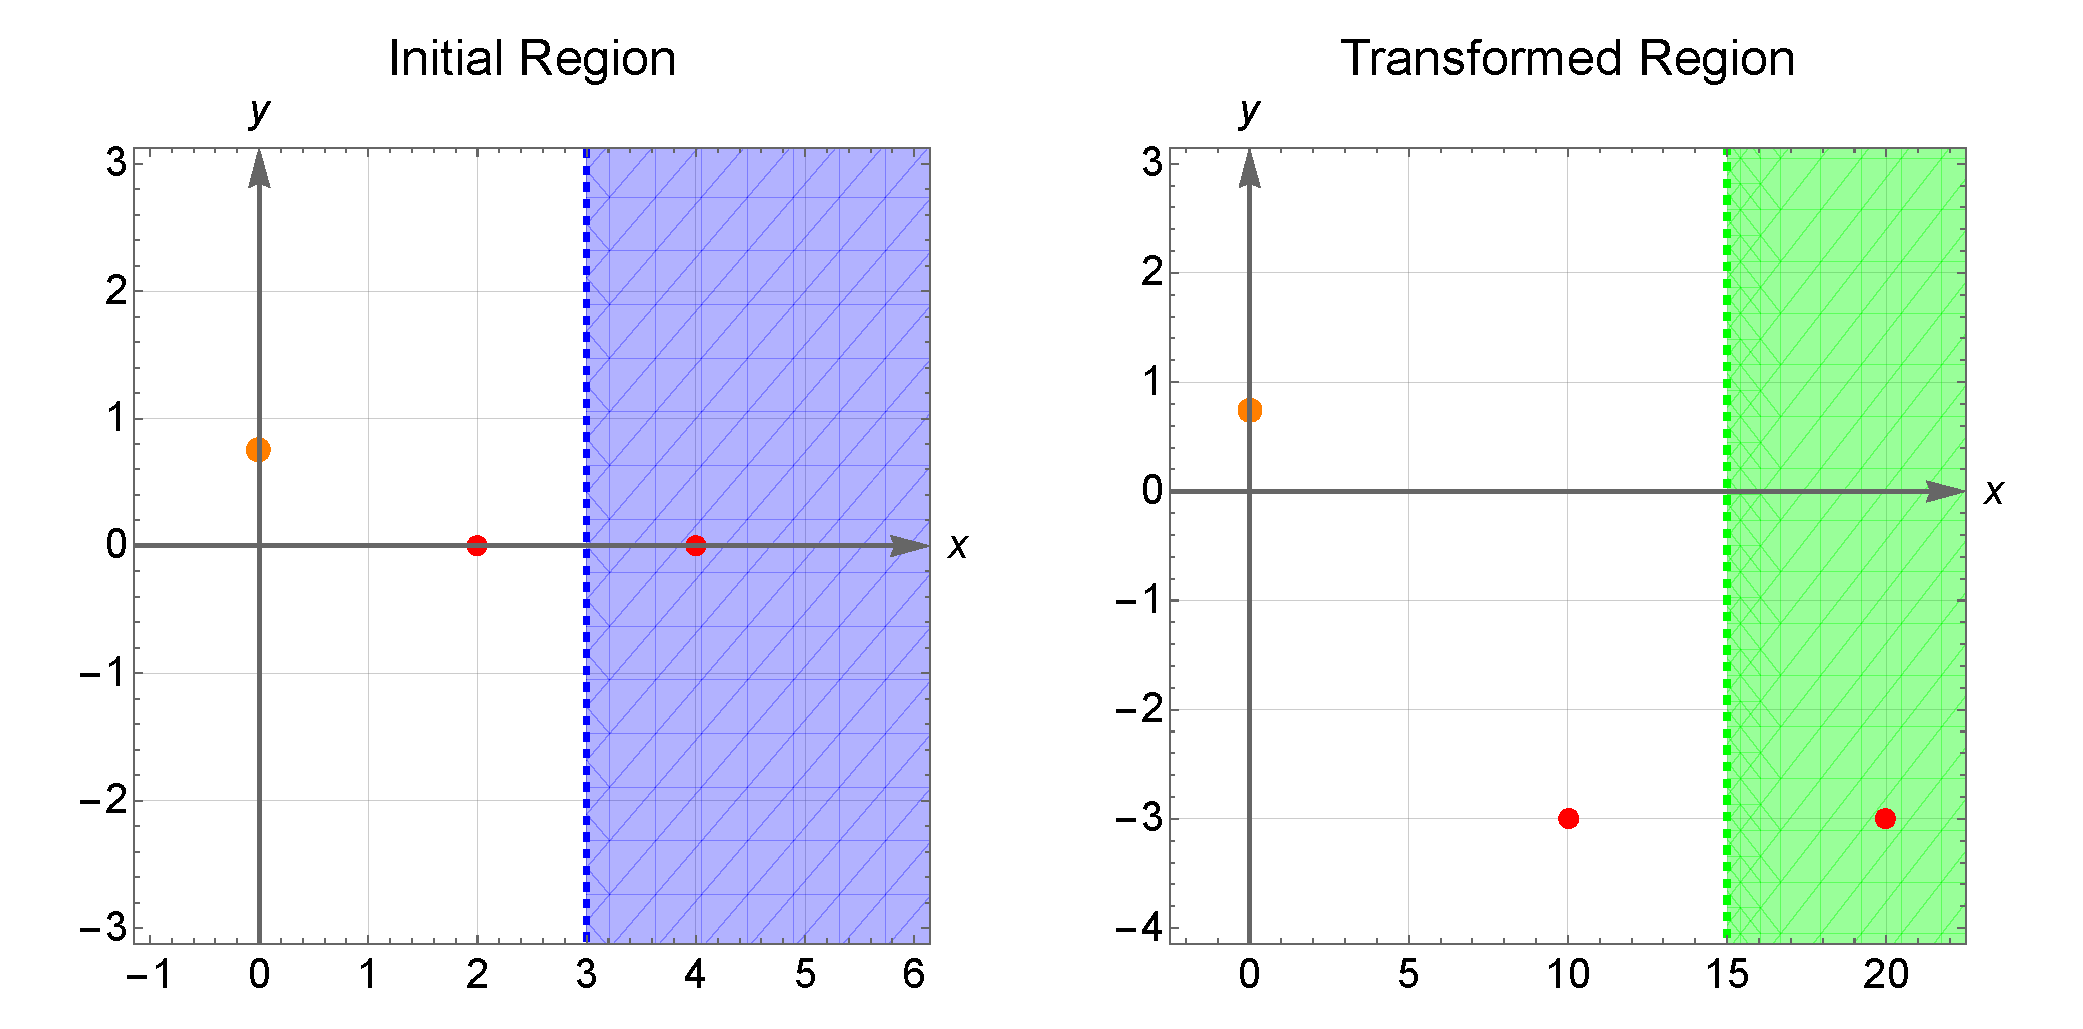
\includegraphics[width=\textwidth]{images/hw_4/problem_1(a).pdf}
    \caption{Відображення $\omega(z)=5z-3i$ на область $\text{Re}(z)>3$.}
    \label{fig:1(a)}
\end{figure}

\vspace{5px}
\textbf{Відображення $\boldsymbol{\omega(z)=\frac{2}{z-1}}$.} 

\textcolor{ForestGreen}{\textit{Образ.}} Оскільки лінійно-дробове відображення переводить узагальнене коло у узагальнене коло, то образом має бути або пряма, або коло. Бачимо, що особлива точка $z=1$ не знаходиться на $\overline{\mathcal{D}}$, тому на виході маємо отримати коло. 

Щоб знайти центр, скористаємося тим, що симетричні точки перетворюються у симетричні під дією $\omega$. Тоді, обираємо $z=1$ -- особлива точка (полюс) $\omega$. Симетричною відносно $\partial\mathcal{D}$ є $z=5$. Отже, маємо $\omega(1) = \infty, \; \omega(5) = \frac{1}{2}$. Оскільки симетричною точкою до $\infty$ відносно кола є центр кола, то $z=\frac{1}{2}$ і є центром нашого шуканого кола. 

Щоб знайти якусь точку на колі, підставимо точку з прямої $\text{Re}(z)=3$, тобто, наприклад, $z=3$. Оскільки $\omega(3) = 1$, то $1 \in \partial\omega(\mathcal{D})$. Отже, рівняння кола стає $\partial\omega(\mathcal{D}):|z-\frac{1}{2}| = \frac{1}{2}$. Залишилося визначитися зі штриховкою. Підставимо $z=4$, тоді $\omega(4) = \frac{2}{3}$ -- лежить всередині кола, а отже $\omega(\mathcal{D}): |z-\frac{1}{2}| < \frac{1}{2}$. 

\textcolor{orange}{\textit{Нерухомі точки.}} Розв'яжемо $\omega(z)=z$, або $\frac{2}{z-1} = z$, звідки $z^2 - z - 2 =0$, коренями якого є $z_1=2$ та $z_2=-1$ -- дві нерухомі точки.

\textcolor{red}{\textit{Симетричні точки.}} Оскільки $\frac{1}{2}$ та $\infty$ є дещо тривіальними точками, підставим ще дві. Візьмемо $z=2$ та $z=4$, наприклад. Тоді матимемо $\omega(4)=\frac{2}{3}, \omega(2) = 2$ -- дві симетричні точки.

Результат зображено на Рисунку \ref{fig:1(b)}.

\begin{figure}
    \centering
    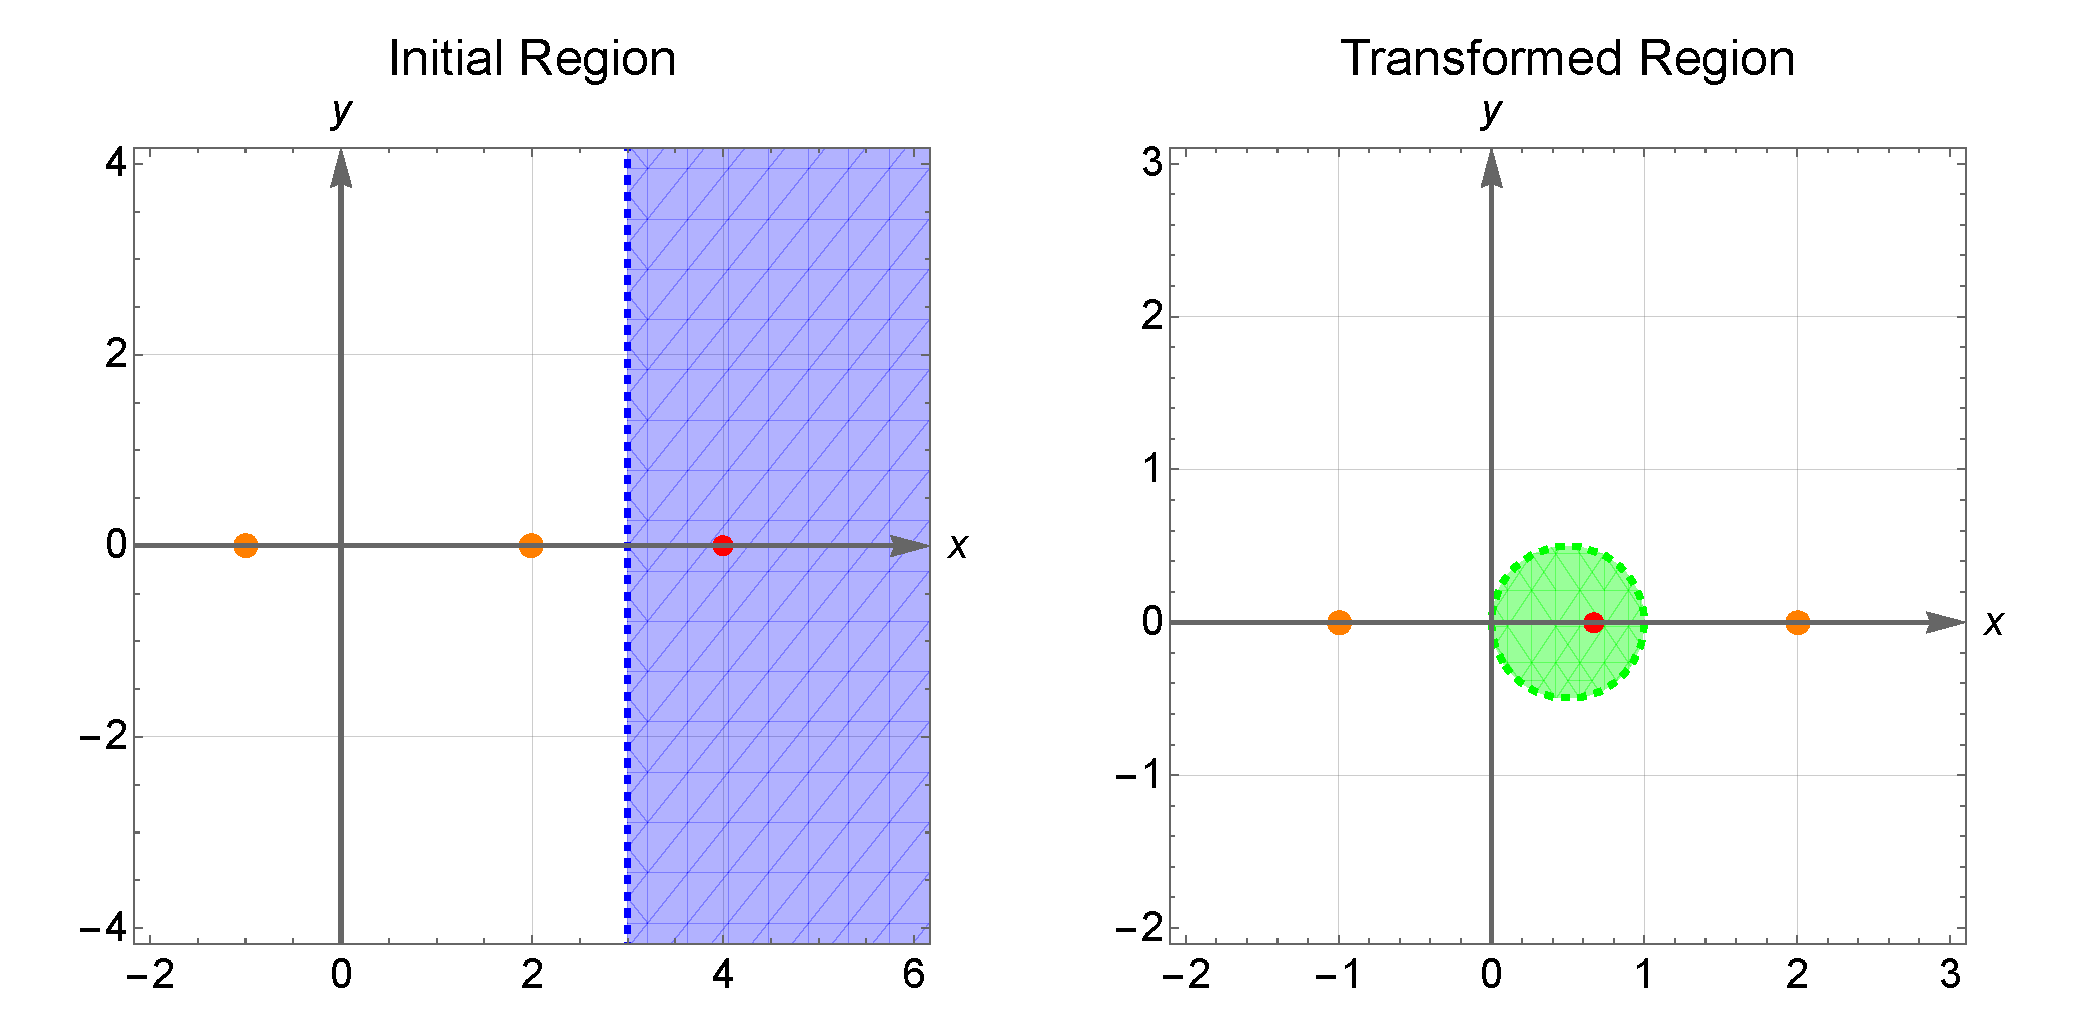
\includegraphics[width=\textwidth]{images/hw_4/problem_1(b).pdf}
    \caption{Відображення $\omega(z)=\frac{2}{z-1}$ на область $\text{Re}(z)>3$. Точка $z=2$ є і нерухомою, і симетричною.}
    \label{fig:1(b)}
\end{figure}

\vspace{10px}
\textbf{Пункт 2.}

\textbf{Відображення $\boldsymbol{\omega(z)=5z-3i}$.}

\textcolor{ForestGreen}{\textit{Образ.}} Лінійне перетворення має перевести коло у коло, але з іншим центром і радіусом. Щоб визначити центр, достатньо лише підставити координати центра: $\omega(-1) = -5-3i$. Отже, $z=-5-3i$ є новим центром. Також, множення на $5$ збільшує радіус вдвічі (в цьому можна впевнитись, наприклад, знайшовши $\omega(1) = 5-3i$ для точки $z=1$, що належить $\partial\mathcal{D}$, і помітити, що радіус дорівнює $|\omega(1)-\omega(-1)|=10$). Також, орієнтація області не змінюється. Отже, образ:
\begin{equation}
    \omega(\mathcal{D}) = \{z \in \mathbb{C}: |z+5+3i| < 10\}
\end{equation}

\textcolor{orange}{\textit{Нерухомі точки.}} Як було показано, єдина нерухома точка -- $z=\frac{3i}{4}$.

\textcolor{red}{\textit{Симетричні точки.}} Візьмемо $z=0$, симетрична ній відносно $\partial\mathcal{D}$ є така точка $z^*$, що $(z-z_0)(z^*-z_0) = R^2$ (оскільки ми на дійсній вісі), де $z_0=-1,R=2$. Отже, підставляючи, маємо $z^*+1=4$, тому $z^*=3$.

Перетворення $\omega$ залишить ці точки симетричними, тому знаходимо $\omega(0)=-3i, \omega(3)=15-3i$ -- дві симетричні точки відносно $\partial\omega(\mathcal{D})$.

Результат зображено на Рисунку \ref{fig:2(a)}.

\begin{figure}
    \centering
    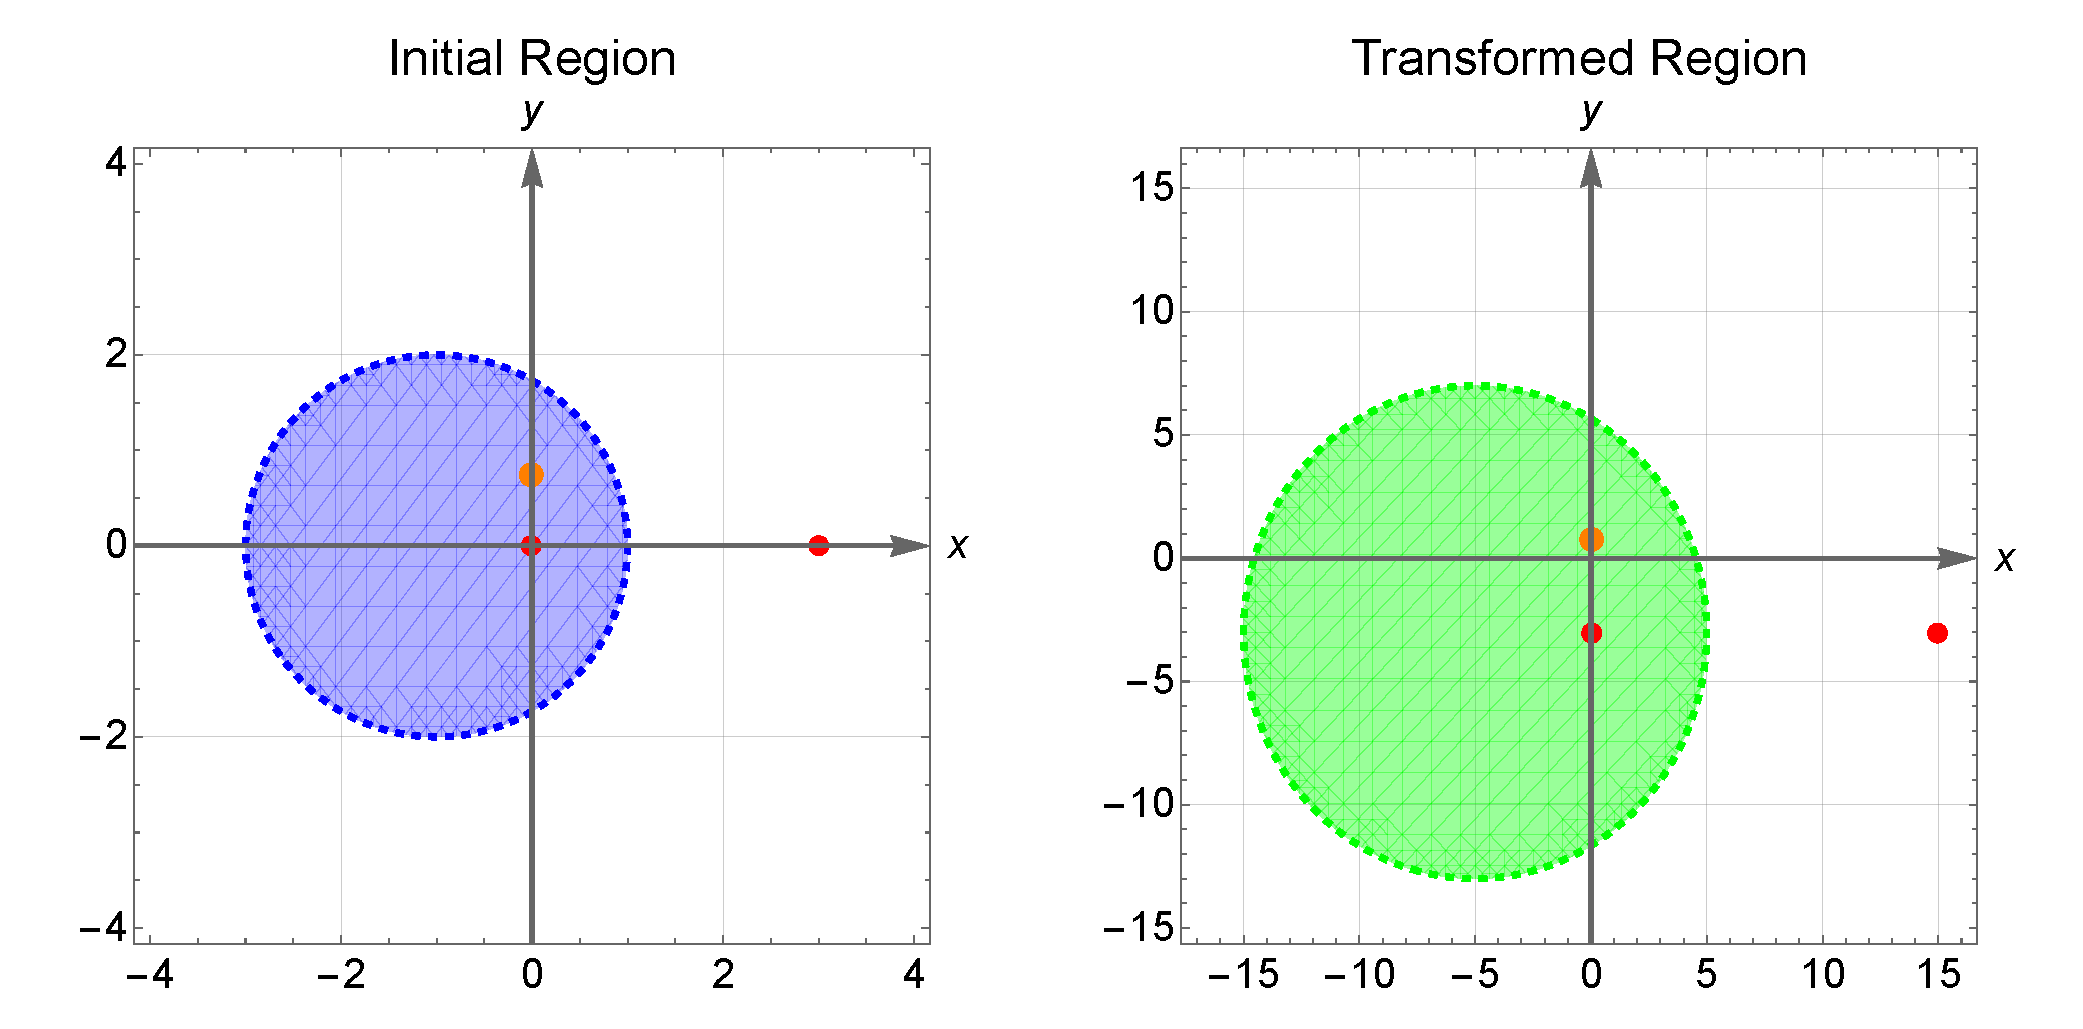
\includegraphics[width=\textwidth]{images/hw_4/problem_2(a).pdf}
    \caption{Відображення $\omega(z)=5z-3i$ на область $|z+1|<2$.}
    \label{fig:2(a)}
\end{figure}

\vspace{5px}
\textbf{Відображення $\boldsymbol{\omega(z)=\frac{2}{z-1}}$.}

\textcolor{ForestGreen}{\textit{Образ.}} Як вже було оговорено, $\omega(\mathcal{D})$ має бути або іншим колом, або прямою. Оскільки особлива точка $z=1$ належить $\partial\mathcal{D}$, то образом має бути пряма. Для того, щоб визначити яка сама пряма, достатньо лише визначити дві точки. Для цього візьмемо якісь дві точки на границі $\partial\mathcal{D}$ і підставимо у наше перетворення $\omega$:
\begin{equation}
    \omega(-1+2i) = \frac{1}{-1+i} = -\frac{1}{2} - \frac{i}{2}, \;\; \omega(-3) = -\frac{1}{2}
\end{equation}

Отже, маємо пряму $\text{Re}(z) = -\frac{1}{2}$. Щоб визначити яка саме частина, просто підставимо якусь точку з області $\mathcal{D}$. Наприклад, $\omega(0) = -2$ лежить ліворуч від $\text{Re}(z) = -\frac{1}{2}$, отже відповіддю буде $\omega(\mathcal{D}) = \{z \in \mathbb{C}: \text{Re}(z) < -\frac{1}{2}\}$. 

\textcolor{orange}{\textit{Нерухомі точки.}} Маємо дві нерухомі точки: $z_1=2,z_2=-1$.

\textcolor{red}{\textit{Симетричні точки.}} $\omega$ переводить симетричні точки у симетричні, тому візьмемо, наприклад, $z_1=0$ та $z_2=3$ -- ми їх брали у попередньому прикладі. Вони переводяться у $\omega(z_1)=-2$ та $\omega(z_2)=1$ -- вони є дійсно симетричними $\text{Re}(z)=-\frac{1}{2}$, оскільки відстань обох до цієї прямої дорівнює $\frac{3}{2}$.

Результат зображено на Рисунку \ref{fig:2(b)}.

\begin{figure}
    \centering
    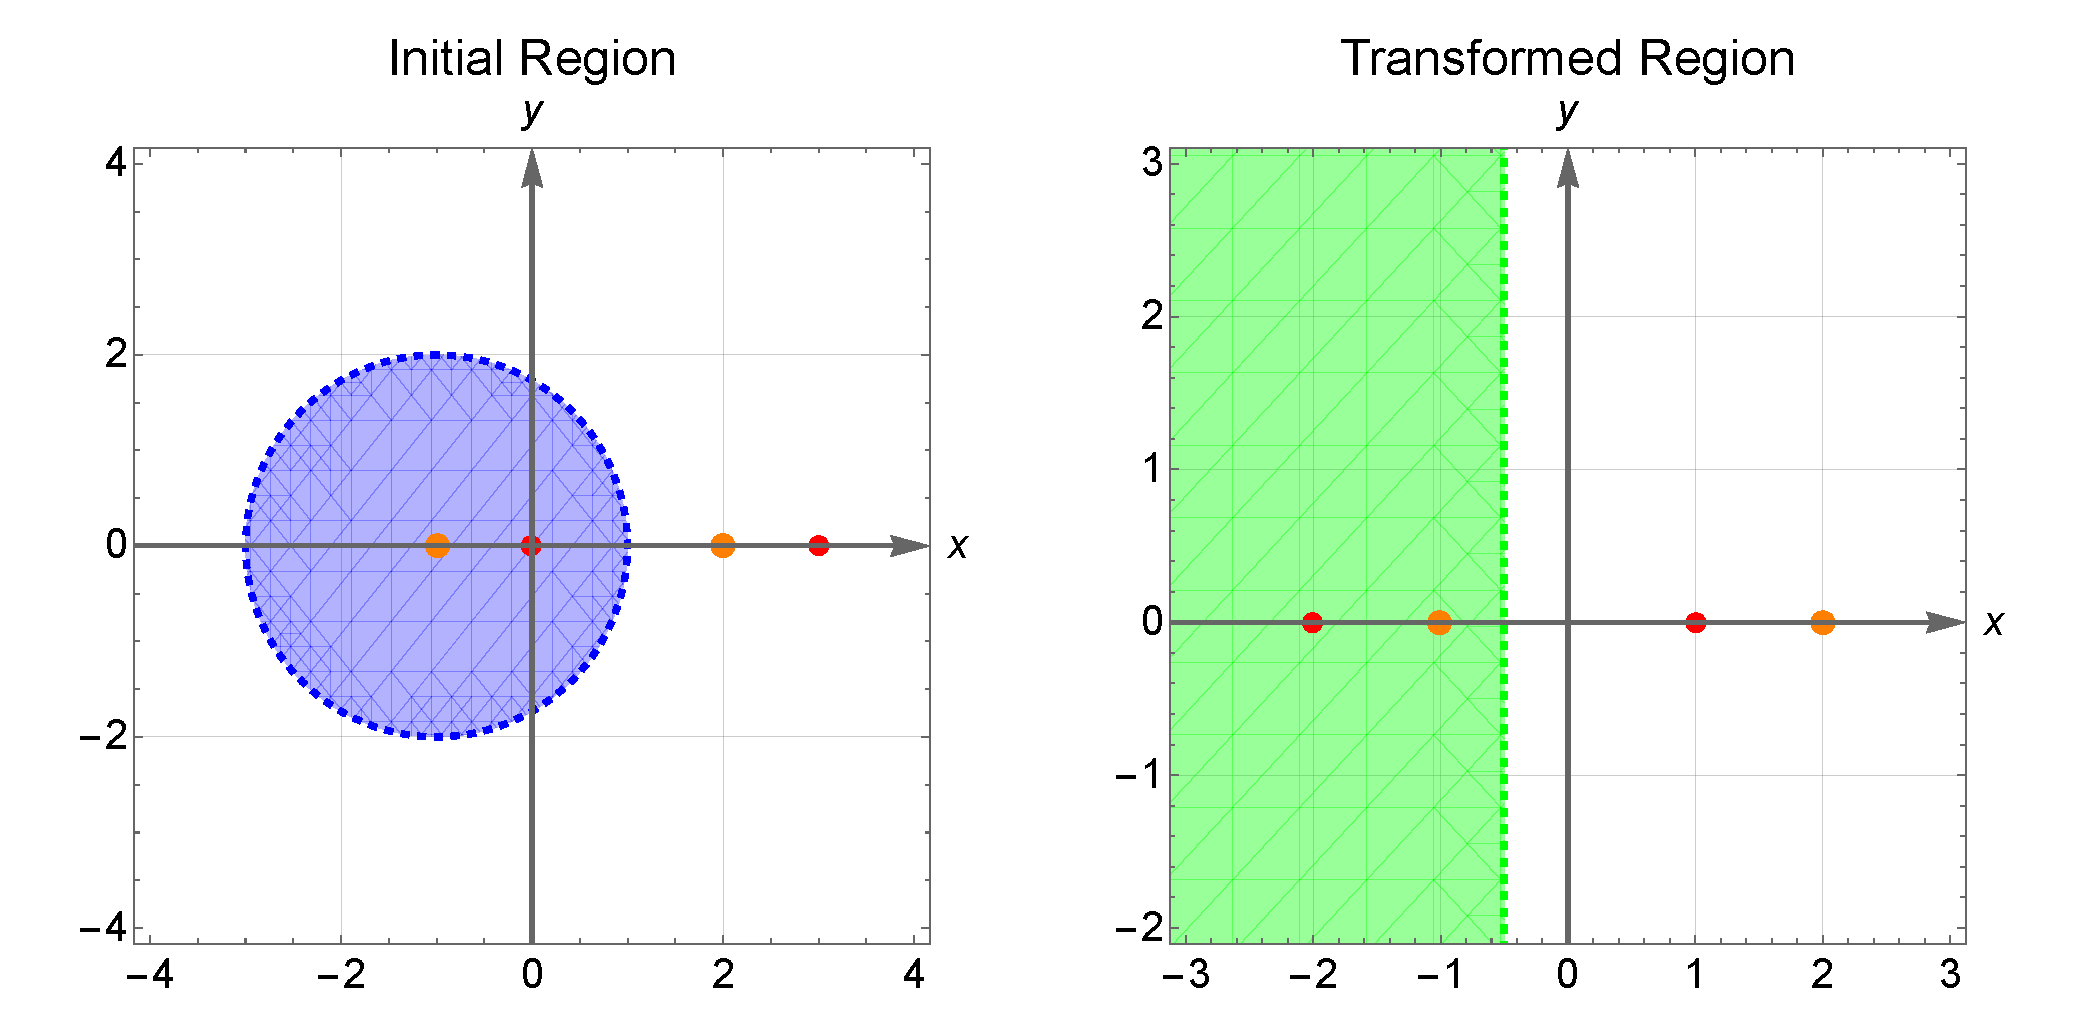
\includegraphics[width=\textwidth]{images/hw_4/problem_2(b).pdf}
    \caption{Відображення $\omega(z)=\frac{2}{z-1}$ на область $|z+1|<2$.}
    \label{fig:2(b)}
\end{figure}

\end{document}
